\newpage
\section{Exercises: Infinite Impulse Response Filters}

\begin{enumerate}

\item Consider the following linear time-invariant system $y[n]=\mathcal{T}\{x[n]\}$, which is defined as:
\begin{equation}
y[n] = y[n-1] + y[n-2] + x[n-1]
\label{eq:exdiffeq}
\end{equation}

\begin{enumerate}[a)]

 \item Assuming that $h[n] = 0$ when $n < 0$, show that the first six values of the impulse response $h[n]=\mathcal{T}\{\delta[n]\}$ of the system defined in Equation \ref{eq:exdiffeq} are:
 \begin{equation*}
h[0] = 0~~~~h[1] = 1~~~~h[2] = 1~~~~h[3] = 2~~~~h[4] = 3~~~~h[5] = 5 
 \end{equation*}


\item Would this filter be classified in signal processing jargon as a
  \emph{finite impulse response} filter (FIR), or an \emph{infinite
  impulse response} (IIR) filter?


\item $z$-transform Equation \ref{eq:exdiffeq}. Use $Y(z)=\mathcal{Z}\{y[n]\}$ and $X(z)=\mathcal{Z}\{x[n]\}$.

\item Show that the system function $\mathcal{H}(z)$ that corresponds to the system defined in Equation \ref{eq:exdiffeq} can be written as:
\begin{equation*}
\mathcal{H}(z)=\frac{z^{-1}}{(1-\varphi_1 z^{-1})(1-\varphi_2 z^{-1})}    
\end{equation*}
Remember that the output of a linear time invariant system in frequency domain is: $Y(z)=\mathcal{H}(z)X(z)$.


\item Determine the values of $\varphi_1$ and $\varphi_2$.

\item The impulse response $h[n]$ of the system defined in Equation \ref{eq:exdiffeq} corresponds to the \emph{\index{Fibonacci sequence}{Fibonacci sequence}}. Provide a closed form formula for the Fibonacci sequence without using recursion. Hint: $h[n] = \mathcal{Z}^{-1}\{\mathcal{H}(z)\}$. You can check your result by comparing the first few values of the sequence $h[0]=0$, $h[1]=1$, $h[2]=1$, $\cdots$.


\item Is the system described in Equation \ref{eq:exdiffeq} bounded-input bounded-output (BIBO) stable? In other words, does the system provide a bounded output for every bounded input? Justify your answer.

\end{enumerate}


\item A time-shifted unit impulse signal is given by: $x[n]=\delta[n-n_0]$. The $z$-transform of this signal is $X(z)=z^{-n_0}$. What is the discrete-time Fourier transform of $x[n]$?


\item Determine the inverse $z$-transforms of the following:
\begin{enumerate}[a)]
\item $A(z)=\frac{1+2z^{-2}}{1-0.25z^{-1}}$
\item $B(z)=\frac{3}{1-0.3z^{-1}} - \frac{2}{1+0.7z^{-1}}$
\item $C(z)=\frac{1+2z^{-2}}{1-0.4z^{-1}-0.32 z^{-2}}$
\end{enumerate}


\item The output of a filter is given by the first-order difference equation:
\begin{equation}
y[n]=0.8y[n-1]+5x[n]
\label{eq:sysfun_ex_iir}
\end{equation}
\begin{enumerate}[a)]
\item What type of filter is this (IIR or FIR)?
\item Find the system function $\mathcal{H}(z)$ of the filter described by equation \ref{eq:sysfun_ex_iir}.
\item Provide a pole-zero plot of $\mathcal{H}(z)$. Is this system stable or not? Explain why.
\item Find the corresponding impulse response $h[n]$.
\item Is this filter a high-pass filter, band-pass filter, or a low-pass filter? Briefly explain why.
\item Let the input signal fed into the system by given by:
\begin{equation}
x[n]=u[n]
\end{equation}
Find the output $y[n]$.
\end{enumerate}


\begin{figure}[!h]
\begin{center}
\begin{minipage}{0.32\textwidth}
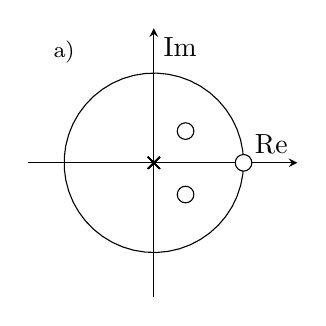
\begin{tikzpicture}
	\begin{axis}[axis equal, ymin=-1.4,xmin=-1.4,ymax=1.4,xmax=1.6,  ticks=none,
    xlabel=$\mathrm{Re}$,
    ylabel=$\mathrm{Im}$, axis lines = center, width=5cm, height=5cm]
	\addplot [black,domain=0:2*pi,samples=50]({cos(deg(x))},{sin(deg(x))});
    \addplot [black, mark = *, fill=white, mark size=3pt] coordinates {( {0.5*cos(45)}, {0.5*sin(45)} )} {};   
      \addplot [black, mark = *, fill=white, mark size=3pt] coordinates {( {0.5*cos(-45)}, {0.5*sin(-45)} )} {};   
            \addplot [black, mark = *, fill=white, mark size=3pt] coordinates {( {1.0*cos(0)}, {1.0*sin(0)} )} {}; 
    \node at (axis cs:-1,1) [above, font={\footnotesize}]{a)};
    \addplot [black, mark = x,mark size=3pt,  only marks] ( {0.0*cos(0)}, {0*sin(0)});   
\end{axis}
\end{tikzpicture}
\end{minipage}
\begin{minipage}{0.32\textwidth}
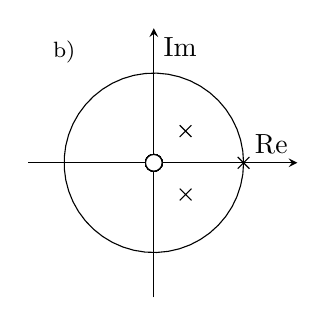
\begin{tikzpicture}
	\begin{axis}[axis equal, ymin=-1.4,xmin=-1.4,ymax=1.4,xmax=1.6,  ticks=none,
    xlabel=$\mathrm{Re}$,
    ylabel=$\mathrm{Im}$, axis lines = center, width=5cm, height=5cm]
	\addplot [black,domain=0:2*pi,samples=50]({cos(deg(x))},{sin(deg(x))});
    \addplot [black, mark = x,mark size=3pt] coordinates {( {0.5*cos(45)}, {0.5*sin(45)} )} {};   
      \addplot [black, mark = x,mark size=3pt] coordinates {( {0.5*cos(-45)}, {0.5*sin(-45)} )} {};   
            \addplot [black, mark = x,mark size=3pt] coordinates {( {1.0*cos(0)}, {1.0*sin(0)} )} {}; 
    \node at (axis cs:-1,1) [above, font={\footnotesize}]{b)};
    \addplot [black, mark = *, fill=white, mark size=3pt,  only marks] ( {0.0*cos(0)}, {0*sin(0)});   
\end{axis}
\end{tikzpicture}
\end{minipage}
\begin{minipage}{0.32\textwidth}
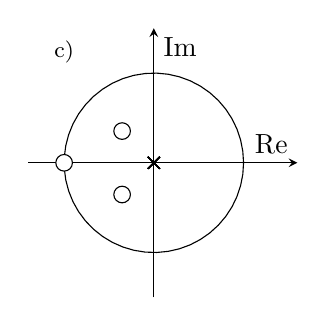
\begin{tikzpicture}
	\begin{axis}[axis equal, ymin=-1.4,xmin=-1.4,ymax=1.4,xmax=1.6,  ticks=none,
    xlabel=$\mathrm{Re}$,
    ylabel=$\mathrm{Im}$, axis lines = center, width=5cm, height=5cm]
	\addplot [black,domain=0:2*pi,samples=50]({cos(deg(x))},{sin(deg(x))});
    \addplot [black, mark = *,fill=white,mark size=3pt] coordinates {( {0.5*cos(135)}, {0.5*sin(135)} )} {};   
      \addplot [black, mark = *, fill=white, mark size=3pt] coordinates {( {0.5*cos(-135)}, {0.5*sin(-135)} )} {};   
            \addplot [black, mark = *, fill=white, mark size=3pt] coordinates {( {1.0*cos(180)}, {1.0*sin(180)} )} {}; 
    \node at (axis cs:-1,1) [above, font={\footnotesize}]{c)};
    \addplot [black, mark = x,mark size=3pt,  only marks] ( {0.0*cos(180)}, {0*sin(180)});   
\end{axis}
\end{tikzpicture}
\end{minipage}
\end{center}
\caption{Three different pole-zero diagrams. The unit circle $z=e^{i\hat{\omega}}$ is marked in each diagram with a solid black line. The zeros of the system function $\mathcal{H}(z)$ are marked with circles (o) and the locations of the poles are marked with crosses (x). The real and imaginary components of poles and zeros only consist of the following numbers: $0, \pm 1$, or $\pm (2\sqrt{2})^{-1}$.}
\label{fig:exzone}
\end{figure}

\item A system function $\mathcal{H}(z)$ is the $z$-transform of the impulse response of a discrete-time LTI system. Figure \ref{fig:exzone} shows pole-zero diagrams that characterize three system functions: \ref{fig:exzone}a), \ref{fig:exzone}b) and \ref{fig:exzone}c). Answer the following questions related to these three pole-zero diagrams. Justify your answers.

\begin{enumerate}[a)]

\item Sketch an approximate magnitude response for the three LTI systems shown
in Figure \ref{fig:exzone}. Use normalized angular frequency $\hat{\omega}$
in units of radians per sample on the x-axis and the magnitude
response $|\mathcal{H}(\hat{\omega})|$ of the y-axis.


\item  Which one of the pole-zero diagrams corresponds to:
\begin{equation}
\mathcal{H}(z) = \frac{(z+1)(z-\alpha)(z-\alpha^*)}{z^3}.
\end{equation}
Here $\alpha=i (2\sqrt{2})^{-1} - (2\sqrt{2})^{-1}$.


\item A low pass filter is a filter that reduces the absolute
amplitude of high frequency spectral components relative to low
frequency spectral components. Which one of the diagrams represents
a \textbf{stable} low-pass filter?

\item Which one of the diagrams represents a \textbf{stable} high-pass filter? 

%\item[(e)] One or more diagrams in Figure \ref{one} correspond to a BIBO unstable filter. Which one(s) are unstable?

\item The filter described in Figure \ref{fig:exzone}c) completely filters out one spectral component of the input signal. What is the frequency of this spectral
component in units of radians per sample.

\item Which of the filters have a finite length impulse response? 
\end{enumerate}


\end{enumerate}